\fancyhead[LE]{\fontsize{8.5pt}{10pt}\selectfont\textbf{\textsf{\thepage}}\quad \textbf{\textsf{CHƯƠNG 1}}\quad \textsf{Các hàm số và Mô hình}}
\fancyhead[RO]{\fontsize{8.5pt}{10pt}\selectfont\textsf{MỤC 1.1}\quad \textbf{\textsf{\thepage}}}

\noindent
\begin{minipage}[t]{0.265\textwidth}
    \fontsize{8pt}{10.5pt}\selectfont
    \vspace{3pt}
    \raggedright
    \textbf{\textsf{HÌNH 14}}

    \vspace{3pt}
    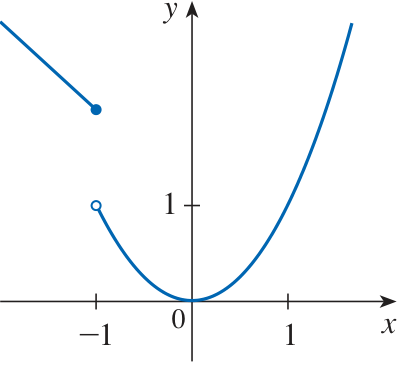
\includegraphics[width=0.82\linewidth]{images/p0049_fig15.png}\\[4pt]
    \textbf{\textsf{HÌNH 15}}

    \vspace{3pt}
    Để ôn tập kỹ hơn về giá trị tuyệt đối, xem Phụ lục A.
\end{minipage}%
\hfill
\begin{minipage}[t]{0.708\textwidth}
    \fontsize{8.8pt}{11.5pt}\selectfont
    Chẳng hạn, parabol $x = y^2 - 2$ được biểu diễn trong Hình 14(a) không phải là đồ thị của một hàm số theo $x$ bởi vì, như bạn có thể thấy, có những đường thẳng đứng cắt parabol tại hai điểm. Tuy nhiên, parabol này lại chứa đồ thị của \textit{hai} hàm số theo $x$. Chú ý rằng phương trình $x = y^2 - 2$ dẫn đến $y^2 = x + 2$, do đó $y = \pm\sqrt{x + 2}$. Vì vậy, nửa trên và nửa dưới của parabol lần lượt là đồ thị của các hàm số $f(x) = \sqrt{x + 2}$ [từ Ví dụ 6(a)] và $g(x) = -\sqrt{x + 2}$. [Xem Hình 14(b) và (c).]

    \begin{center}
        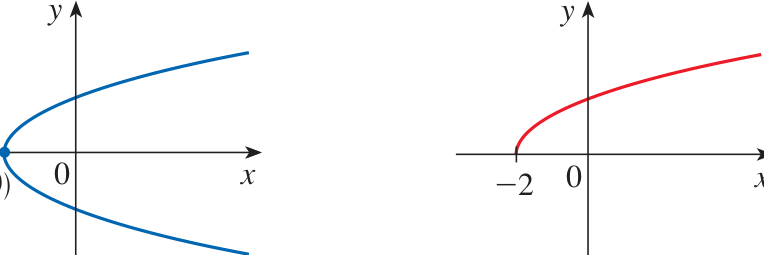
\includegraphics[width=\linewidth]{images/p0049_fig14.png}
    \end{center}

    Ta nhận thấy rằng nếu hoán đổi vai trò của $x$ và $y$, thì phương trình $x = h(y) = y^2 - 2$ \textit{thực sự} xác định $x$ là một hàm số theo $y$ (với $y$ là biến độc lập và $x$ là biến phụ thuộc). Đồ thị của hàm số $h$ chính là parabol trong Hình 14(a).

    \vspace{0.6em}
    \noindent{\color{stewartcyan}\rule{1.1ex}{1.1ex}}\quad \textbf{\textsf{\large Các hàm số cho bởi nhiều công thức}}

    \vspace{0.3em}
    Các hàm số trong bốn ví dụ sau đây được xác định bởi các công thức khác nhau trên các phần khác nhau của tập xác định. Những hàm số như vậy được gọi là \textbf{hàm số cho bởi nhiều công thức} (hay \textbf{hàm từng khúc}).

    \vspace{0.5em}
    \noindent\textbf{\textsf{\color{stewartcyan}VÍ DỤ 7}}\quad Cho hàm số $f$ được xác định bởi
    \[
    f(x) = \begin{cases} 
    1 - x & \text{nếu } x \leqslant -1 \\ 
    x^2 & \text{nếu } x > -1 
    \end{cases}
    \]
    Tính $f(-2)$, $f(-1)$ và $f(0)$, sau đó vẽ đồ thị của hàm số.

    \vspace{0.4em}
    \noindent\textbf{\textsf{\color{stewartcyan}LỜI GIẢI}}\quad Hãy nhớ rằng một hàm số là một quy tắc. Đối với hàm số cụ thể này, quy tắc như sau: Trước tiên hãy nhìn vào giá trị của đầu vào $x$. Nếu xảy ra trường hợp $x \leqslant -1$, thì giá trị của $f(x)$ là $1 - x$. Mặt khác, nếu $x > -1$, thì giá trị của $f(x)$ là $x^2$. Lưu ý rằng mặc dù hai công thức khác nhau được sử dụng, $f$ chỉ là \textit{một} hàm số, không phải hai.
    \begin{gather*}
    \text{Vì } -2 \leqslant -1, \text{ ta có } f(-2) = 1 - (-2) = 3. \\
    \text{Vì } -1 \leqslant -1, \text{ ta có } f(-1) = 1 - (-1) = 2. \\
    \text{Vì } 0 > -1, \text{ ta có } f(0) = 0^2 = 0.
    \end{gather*}

    Làm thế nào để ta vẽ đồ thị của $f$? Ta nhận thấy rằng nếu $x \leqslant -1$, thì $f(x) = 1 - x$, vì vậy phần đồ thị của $f$ nằm ở bên trái đường thẳng đứng $x = -1$ phải trùng với đường thẳng $y = 1 - x$, đường thẳng có hệ số góc $-1$ và tung độ gốc là $1$. Nếu $x > -1$, thì $f(x) = x^2$, nên phần đồ thị của $f$ nằm ở bên phải đường thẳng $x = -1$ phải trùng với đồ thị của $y = x^2$, vốn là một parabol. Điều này cho phép ta phác thảo đồ thị như trong Hình 15. Điểm tròn đặc biểu thị điểm $(-1, 2)$ thuộc đồ thị; điểm tròn rỗng biểu thị điểm $(-1, 1)$ không thuộc đồ thị.\hfill{\color{stewartcyan}$\blacksquare$}

    \vspace{0.6em}
    Ví dụ tiếp theo về hàm số cho bởi nhiều công thức là hàm giá trị tuyệt đối. Nhắc lại rằng \textbf{giá trị tuyệt đối} của một số $a$, ký hiệu là $|a|$, là khoảng cách từ $a$ đến 0 trên trục số thực. Khoảng cách luôn dương hoặc bằng 0, vì vậy ta có
    \[
    |a| \geqslant 0 \qquad \text{với mọi số } a
    \]
\end{minipage}